\section{Technische Umsetzung des Protoypen}

Im folgenden Abschnitt wird auf die Implementierung des Alarmszenarios und dazugehörige Überlegungen eingegangen. Zu Beginn wird der gewählte Technologie-Stack dargelegt und durch Ausführungen zur Systemarchitektur ergänzt. 
Daran schließt ein Abschnitt zur Erklärung der Konfigurationen von Alarmszenarien als auch der eingesetzten APIs an.

\subsection{Technologie-Stack}

Die Auswahl des Technologie-Stacks zur Implementierung von ALAARM-ZIP hängt zentral von einer Vielzahl von Vorbedingungen ab.


Bezüglich der verwendeten \textbf{Programmiersprache} wurde sich für den Einsatz von \textit{TypeScript}\footnote{Siehe \href{https://typescriptlang.org/}{https://typescriptlang.org/}} entschieden. Neben der Eignung für Webapplikation und der universellen Verwendbarkeit, d.h. der Möglichkeit, die Anwendung sowohl via Browser (Windows, iPadOS, Linux) als auch serverseitig auszuführen,  waren sprachenspezifische Eigenschaften wie Typisierung für die Projektgruppe entscheidend, um sich auf \textit{TypeScript} festzulegen.

Für das \textbf{Frontend} wurde sich für \textit{NextJS}\footnote{Siehe \href{https://nextjs.org/}{https://nextjs.org/}} als spezifisches \textit{React}-Framework entschieden. Hiermit können Elemente einer Website bereits serverseitig gerendert werden, bevor sie zum Client gesendet werden, ebenso wird ein Routing mitgeliefert. Zusätzlich erfolgt der Einsatz der UI-Komponentenbibliothek \textit{ShadCN}\footnote{Siehe \href{https://ui.shadcn.com/}{https://ui.shadcn.com/}}, welche auf dem CSS-Framework \textit{TailwindCSS}\footnote{Siehe \href{https://tailwindcss.com/}{https://tailwindcss.com/}} basiert. 

Für den \textbf{Controller} wurde sich für die \textit{NodeJS}\footnote{Siehe \href{https://nodejs.org/}{https://nodejs.org/}} Laufzeitumgebung aufgrund der ereignisgesteuerten I/O-Architektur für Echtzeitanwendungen entschieden. \textit{REST APIs} werden beim Controller dafür genutzt, um einen Kommunikationsfluss zwischen Admin-Panel, Client und MQTT-Server zu realisieren (Systemarchitektur siehe Kapitel \ref{chap:systemarchitecture}). Durch die Verbindung mit \textit{MQTT} können Nachrichten unmittelbar an den MQTT-Broker gesendet werden.

Für die \textbf{Entwicklung} wurde ein \textit{git-Repository}\footnote{Siehe \href{https://git-scm.com/}{https://git-scm.com/}} aufgesetzt, welches durch den Anbieter Github\footnote{Siehe \href{https://github.com/}{https://github.com/}} bereitgestellt wird. Das Repository inkl. vollständiger technischer Dokumentation kann unter folgendem Link eingesehen werden:  \url{https://github.com/ToKoSoftware/up-alaarm-zip}. Die Verwaltung des Mono-Repositories erfolgte mit \textit{Lerna}\footnote{Siehe \href{https://lerna.js.org/}{https://lerna.js.org/}}. Zur Paketverwaltung wurde auf \textit{npm}\footnote{Siehe \href{https://npmjs.com/}{https://npmjs.com/}}  zurückgegriffen. Um einen einheitlichen Codestyle zu erzwingen, wurden die Pakete \textit{Prettier}\footnote{Siehe \href{https://prettier.io/}{https://prettier.io/}} und \textit{ESLint}\footnote{Siehe \href{https://eslint.org/}{https://eslint.org/}} genutzt. Mithilfe von \textit{Husky}\footnote{Siehe \href{https://typicode.github.io/husky/}{https://typicode.github.io/husky/}} wurden diese Tools vor jedem Commit automatisiert ausgeführt. Das Deployment auf einem Web-Server des Anbieters \textit{Vercel}\footnote{Siehe \href{https://vercel.com/}{https://vercel.com/}} erfolgt automatisiert on-push auf den \textit{main branch} des git-Repository.


\subsection{Systemarchitektur}
\label{chap:systemarchitecture}
Der folgenden Abbildung ist die Systemarchitektur von ALAARM-ZIP zu entnehmen:

\begin{figure}[h]
   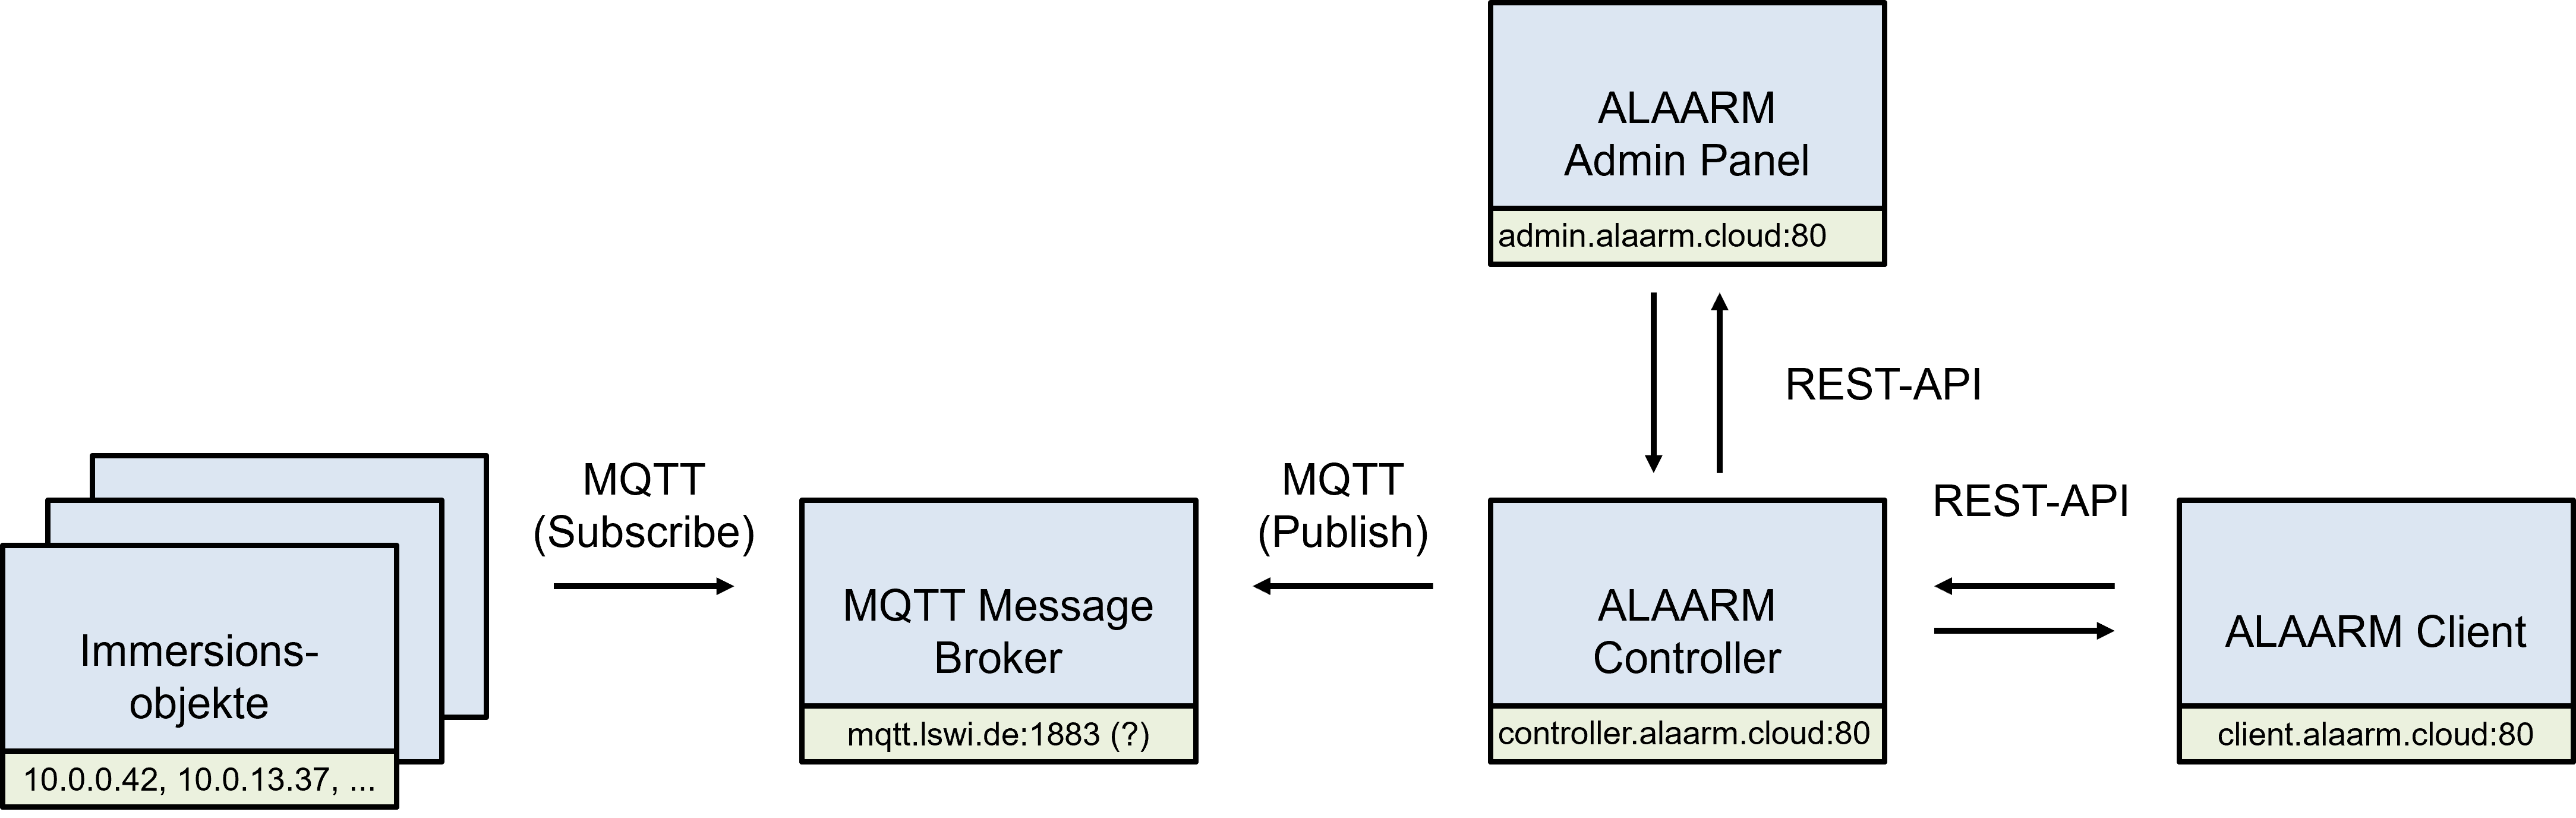
\includegraphics[width=15cm, height=5.87cm]{res/20230809_architecture.png}
   \caption{Systemarchitektur}
\end{figure}


Den Kernkommunikationshub nimmt der \textit{ALAARM Controller} ein, welcher die Kommunikation zwischen dem Admin Panel, dem Client und dem MQTT Message Broker übernimmt. Das Admin Panel ist die Steuerung des Administrators, welcher verantwortlich für die Entwicklung und das Management von Szenarien für die Simulation ist.
Das \textit{Admin Panel} ist auf \href{https://admin.alaarm.cloud/}{https://admin.alaarm.cloud/} bereitgestellt.
Die \textit{ALAARM Client} Komponente verarbeitet die Eingaben auf dem Tablet von Simulationsteilnehmern und bildet die Rätsellogik ab. Ebenso realisiert diese Komponente die QR-Scanner Funktionalität, damit via QR Codes Rätsel durch Simulationsteilnehmer aufgerufen werden können. Bereitgestellt wird der Client auf \href{https://client.alaarm.cloud/}{https://client.alaarm.cloud/}.

Mithilfe des \textit{MQTT Message Brokers} können über den Controller Events übergeben werden, welche durch MQTT an die entsprechend adressierten und angebundenen Immersionsobjekte wie den Subwoofer übergeben werden. Entsprechende Datenobjekte werden durch die \textit{Immersionsobjekte} schlussendlich ausgeführt. Bei Ansteuerung kann ein Subwoofer beispielsweise einen kräftigen Druckstoß durchführen, nachdem ein Rätsel nicht im definierten Zeitrahmen gelöst worden ist und das Szenario eine neue Eskalationsstufe aufruft. 

\subsection{Konfiguration von Alarmszenarien}

Zu Beginn einer geplanten Alarmsimulation kann durch den Administrator das zu durchlaufende Szenario konfiguriert werden. Hierfür ist zunächst die Adresse \href{https://admin.alaarm.cloud}{https://admin.alaarm.cloud} aufzurufen. Mit dem Klick auf den schwarzen Button \textit{\enquote{Szenario starten}} öffnet sich auf der rechten Seite die Seitenleiste zur Konfiguration des Szenarios. Zunächst ist durch den Admin mithilfe eines Unique Resource Identifiers die Adresse des Controllers anzugeben, damit die gewünschte Ablaufsteuerung für die Simulation geladen werden kann. Zur Authentifizierung des Administrators ist als Nächstes das festgelegte Secret einzugeben. Daran schließt das Eingabefeld an, in welches Daten zur Spezifizierung des Szenarios im JSON-Formformat übermittelt werden müssen.
Schlussendlich kann die Simulation des Szenarios über einen Klick des schwarzen Buttons \textit{\enquote{Szenario starten}} in der Seitenleiste begonnen werden.

Dabei empfängt der adressierte Controller die angegebene Konfiguration und beginnt entsprechend der Ablauflogik Messages an die Immersionsgeräte zu verteilen.

\begin{figure}[h]
   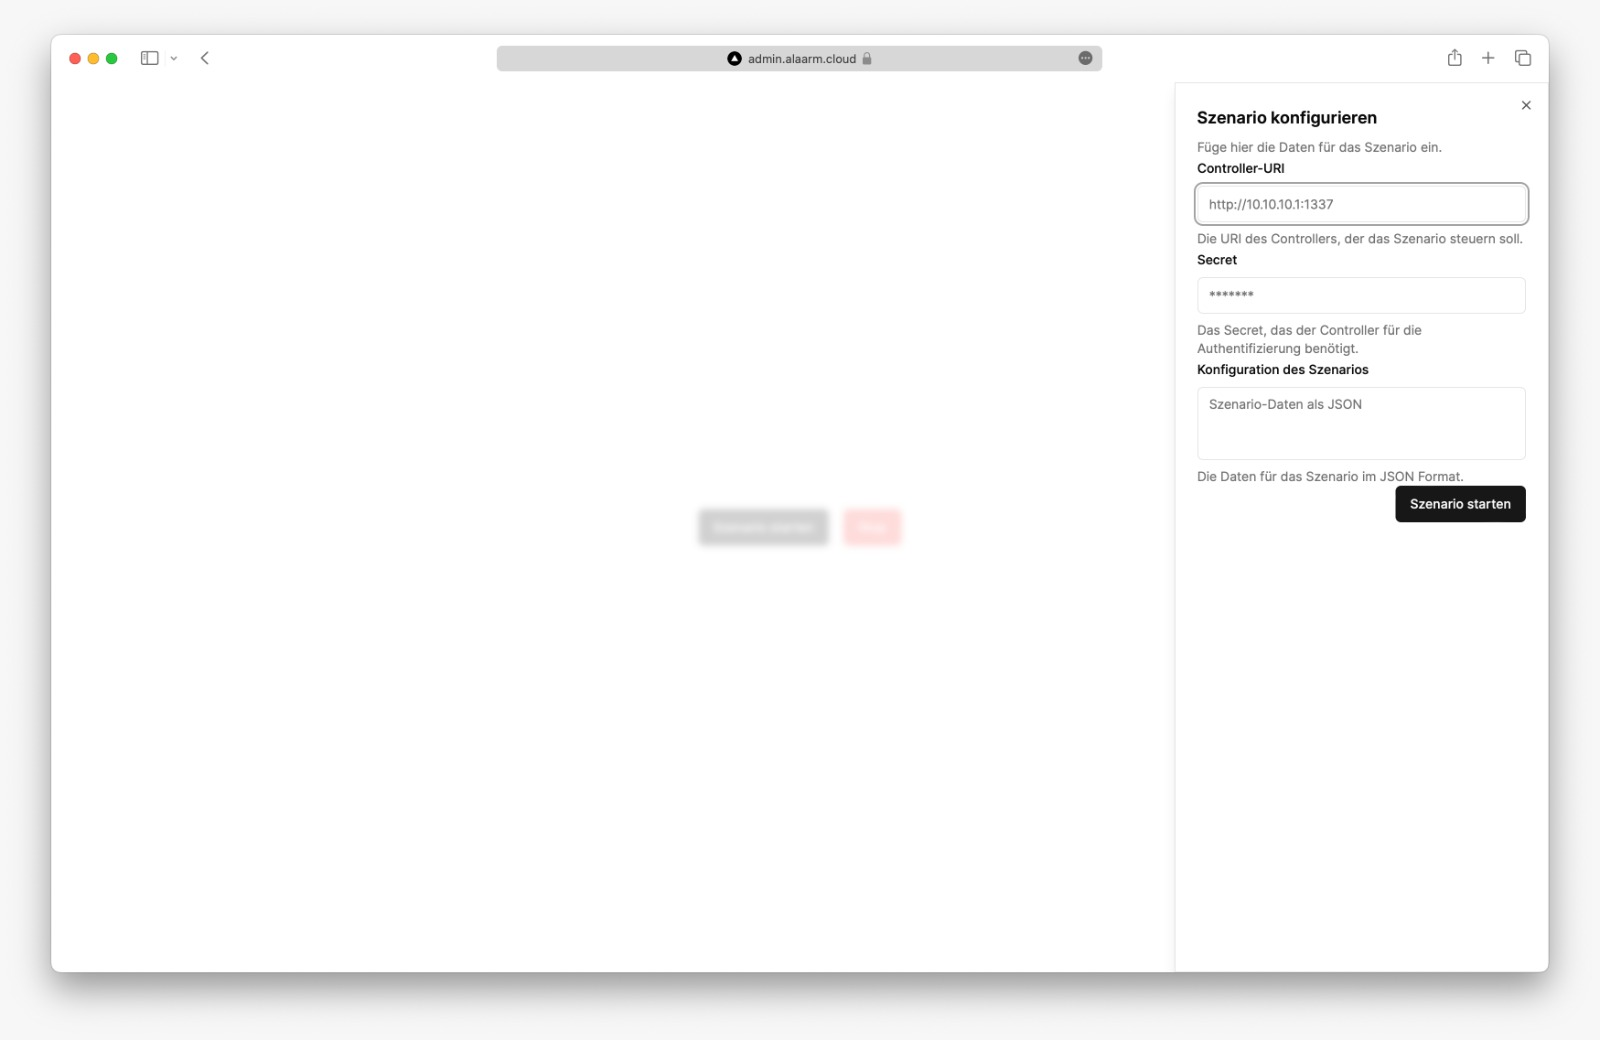
\includegraphics[width=15cm, height=10.87cm]{res/20230821_Szenario_Configuration.jpg}
   \caption{Szenariokonfiguration}
\end{figure}



\newpage
\subsection{APIs}

Zur Kommunikation verschiedener Komponenten untereinander kommen RESTful APIs und das MQTT Message Protocol zum Einsatz. 

Requests via RESTful API verfügen über ein Datenobjekt, welches je nach Anfrage etwa dem Start eines Szenarios (\textit{api/v1/scenario/start}) variabel ausfällt. Der Start und Stopp von Szenarien wird über POST Requests zum Anlegen jener neuen Ressource abgewickelt. Zum Abrufen von Daten wie Rätseln oder dem Status, etwa ob ein Rätsel rechtzeitig gelöst worden ist, werden GET Requests genutzt \autocite{masse2011rest}.

Um Immersionsobjekte zur Auslösung von Immersionseffekten wie Licht und Geräusche anzusteuern, wird das MQTT Message Protocol verwendet. Die Ansteuerung erfolgt über festgelegte \textit{Event Types}. Bei der Ansteuerung wird ein \textit{Payload}, etwa ein Link zu einer .mp3 Datei, übergeben, um von Seite des Immersionsobjekts den gewünschten Effekt auszuführen.
